\section{Chapter 8 -- Datapath and Control}
%%%%%%%%%%%%%%%%%%%%%%%%%%%%%%%%%%%%%%%%%%%%%%%%%%%%
%% Here are the helpfull stuff
%%%%%%%%%%%%%%%%%%%%%%%%%%%%%%%%%%%%%%%%%%%%%%%%%%%%
\subsection{Helpfull Stuff}

\scalebox{0.7}{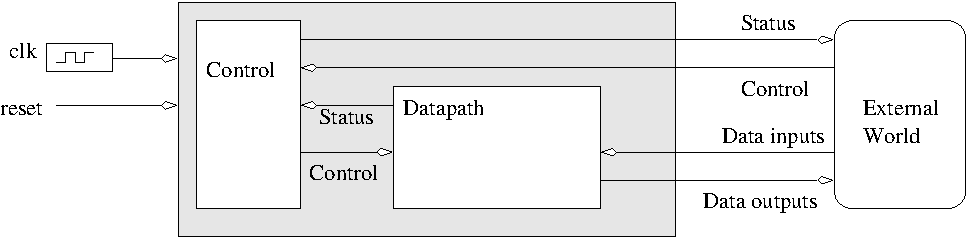
\includegraphics{./Fig8/Abstract}}


Mini-C statements
\begin{itemize}
\item if (condition) then BODY$_1$ else BODY$_2$
\item for (i=A; i$<$B; i $+=$ 1) BODY
\item while(condition) BODY
\item X = value
\end{itemize}
where BODY contains 0 or more statements.
\vspace{0.1in}

\begin{tabular}{|l|l|l|l|l|} \hline
Device      & Data in     & Data out & Status   & Control \\ \hline
N:M Decoder &  1 bit       & M bits  & 	& N bits  \\ \hline
N:1 Mux     & N bits  & 1 bit    & 	&  $\log_2(N)$ bits  \\ \hline
MxNx1 Mux   & N, each M bits  & M bits & 	&  $\log_2(N)$ bits  \\ \hline
N bit adder &  2, each N bits & N bits & Overflow &   \\ \hline
N bit add/sub & 2, each N bits & N bits & Overflow & 1 bit  \\ \hline
N bit comparator  & 2, each N bits &  & 3 bits &   \\ \hline
BCD to 7-segment  & 4-bits & 7-bits & &   \\ \hline
N-bit priority encoder   & N-bits & $\log(N)$-bits & &   \\ \hline
N bit register      & N bits & N bits &  & 1 bit  \\ \hline
N bit shift register &  N bits & N bits &  & 2 bits  \\ \hline
N bit counter       & N bits & N bits &  & 2 bits  \\ \hline
Three state buffer    & N bits & N bits & & 1 bit  \\ \hline
N:M RAM             & $\log_2(N)$ bits, M bits & M bit & & 3 bits  \\ \hline
N-bit Bus transceiver     & N bits & N bits & & 2 bit  \\ \hline
\end{tabular}
\label{page:boxlist}


%%%%%%%%%%%%%%%%%%%%%%%%%%%%%%%%%%%%%%%%%%%%%%%%%%%%
%% Here are terms that the students define
%%%%%%%%%%%%%%%%%%%%%%%%%%%%%%%%%%%%%%%%%%%%%%%%%%%%
%%% \subsection{Definitions}
%%% \begin{description}
%%% \item [Control Word]
%%% \item [Status Word]
%%% \item[Two-line handshake]
%%% \end{description}

\begin{tabular}{|l|l|} \hline
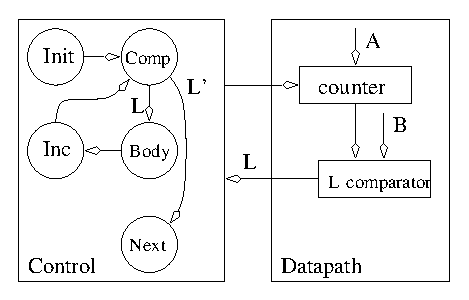
\includegraphics{./Fig8/For}    & 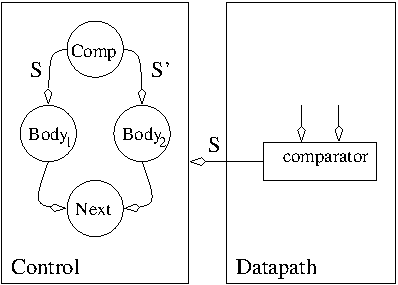
\includegraphics{./Fig8/IfThen}      \\ 
\verb-for(i=A; i<B; i++) BODY-  & \verb+if(condition) BODY1 else BODY2+\\ \hline

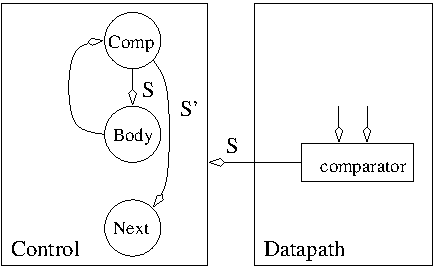
\includegraphics{./Fig8/While}	& 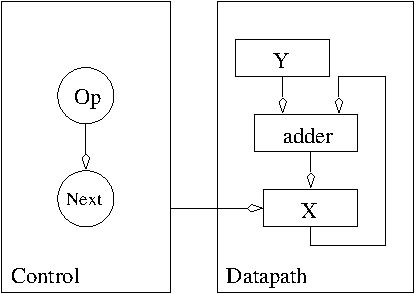
\includegraphics{./Fig8/Op}	\\
\verb+while(condition} BODY+	& \verb+x=value+ 		\\ \hline
\end{tabular}



%%%%%%%%%%%%%%%%%%%%%%%%%%%%%%%%%%%%%%%%%%%%%%%%%%%%
%% Here are the problems
%%%%%%%%%%%%%%%%%%%%%%%%%%%%%%%%%%%%%%%%%%%%%%%%%%%%
\subsection{Problems}
\begin{description}


\item[Minimum Search]

Design a digital circuit that looks for the smallest 
8-bit integer in a 128x8 bit RAM.  The numbers
are stored at addresses $0\ldots 99$, you may assume that the 
RAM is preloaded with data.

\begin{verbatim}
1.  min = 0xFF;               // Set the min reg to largest value
2.  for (i=0; i<100; i++) {   // Search through the entire array
3.      MBR=RAM[i];           // read an 8-bit value from the RAM
4.      if (MBR<min) then     // If MBR is smaller than min
5.          min = MBR;        //   then set min to the smallest value
6   } // end for
\end{verbatim}


\scalebox{0.7}{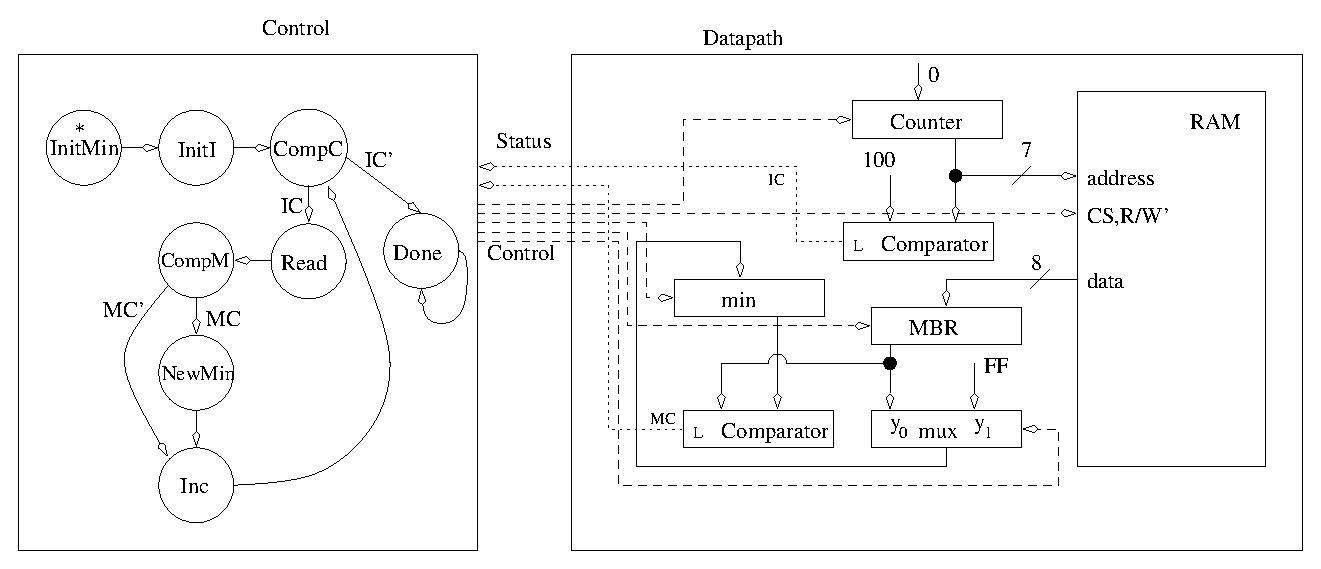
\includegraphics{./Fig8/MinSearch}}


\begin{tabular}{c||c|c|c|c|c|c|c}  
State   & CS       & RE     &  WE      &  Reg Min  & Min mux       & Counter & MBR	\\ \hline
        & 0 off    & 0 idle & 0 idle   &  0 hold   & 0 load FF     & 00 hold & 0 hold	\\ \hline
        & 1 active & 1 read & 1 write  &  1 load   & 1 load MBR    & 01 load & 1 load	\\ \hline
        &          &       &           &           &               & 10 count& 		\\ \hline
        &          &       &           &           &               & 11 reset& \\ \hline \hline
InitMin &         &      &          &          &              &       &    \\ \hline
InitI   &         &      &          &          &              &       &    \\ \hline
CompC   &         &      &          &          &              &       &    \\ \hline
Read    &         &      &          &          &              &       &    \\ \hline
CompM   &         &      &          &          &              &       &    \\ \hline
NewMin  &         &      &          &          &              &       &    \\ \hline
Inc     &         &      &          &          &              &       &    \\ \hline
Done    &         &      &          &          &              &       &    \\ 
\end{tabular}

\begin{tabular}{p{2in}p{1in}}
$D_{IM} =$	&	$Z_{CS} =$  		\\
$D_{II} =$ 	&	$Z_{RE} =$ 		\\
$D_{CC} =$	&	$Z_{WE} =$  		\\
$D_{R} = $	&	$Z_{RM} =$ 		\\
$D_{CM} =$ 	&	$Z_{MM} =$ 		\\
$D_{NM} =$ 	&	$Z_{C1} =$ 		\\
$D_{I} = $	&	$Z_{C0} =$ 		\\
$D_{D} = $	&	$Z_{MBR} =$ 		\\
\end{tabular}

\pagebreak
Shade the active FF and any BBBs which are read or written.

\begin{tabular}{ll}
\scalebox{0.3}{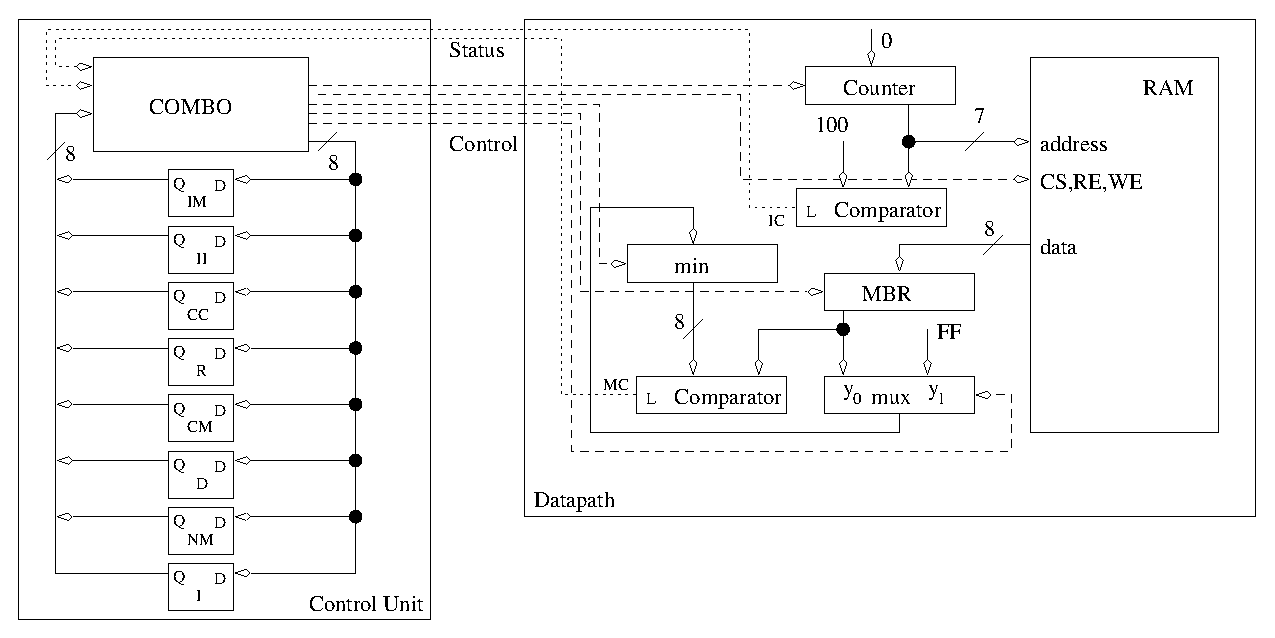
\includegraphics{./Fig8/MinSearch2}} & 
	\scalebox{0.3}{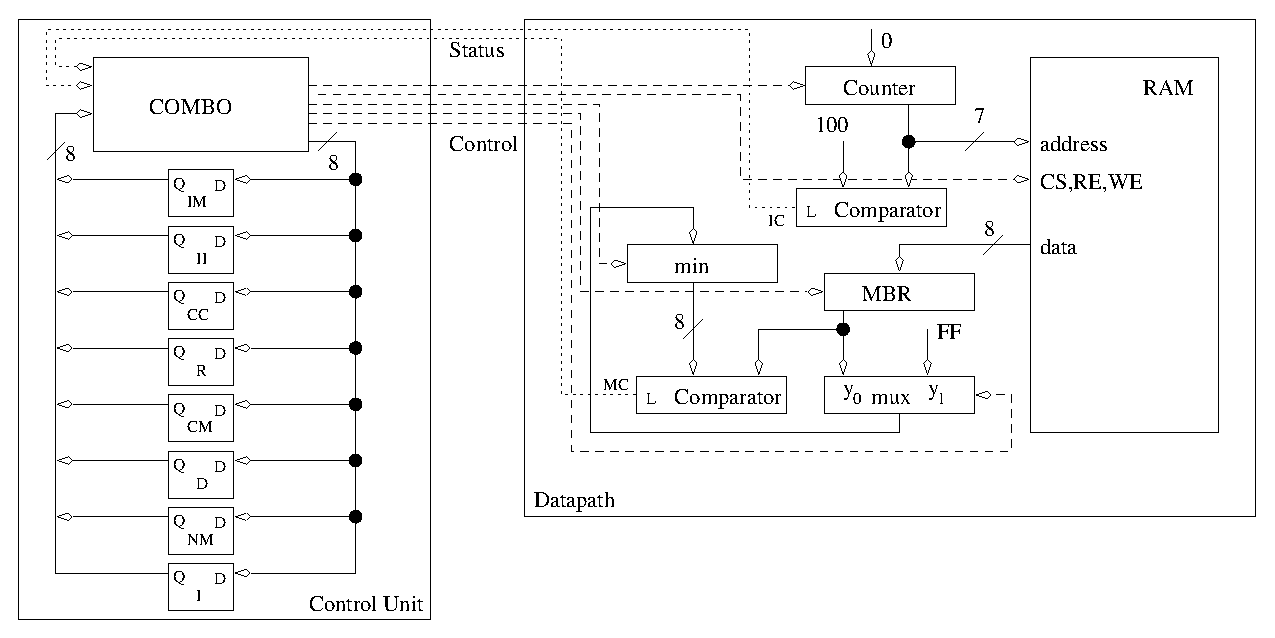
\includegraphics{./Fig8/MinSearch2}} \\
1. State {\bf InitMin} \vspace{10mm}        & 5. State {\bf CompM} \\
\scalebox{0.3}{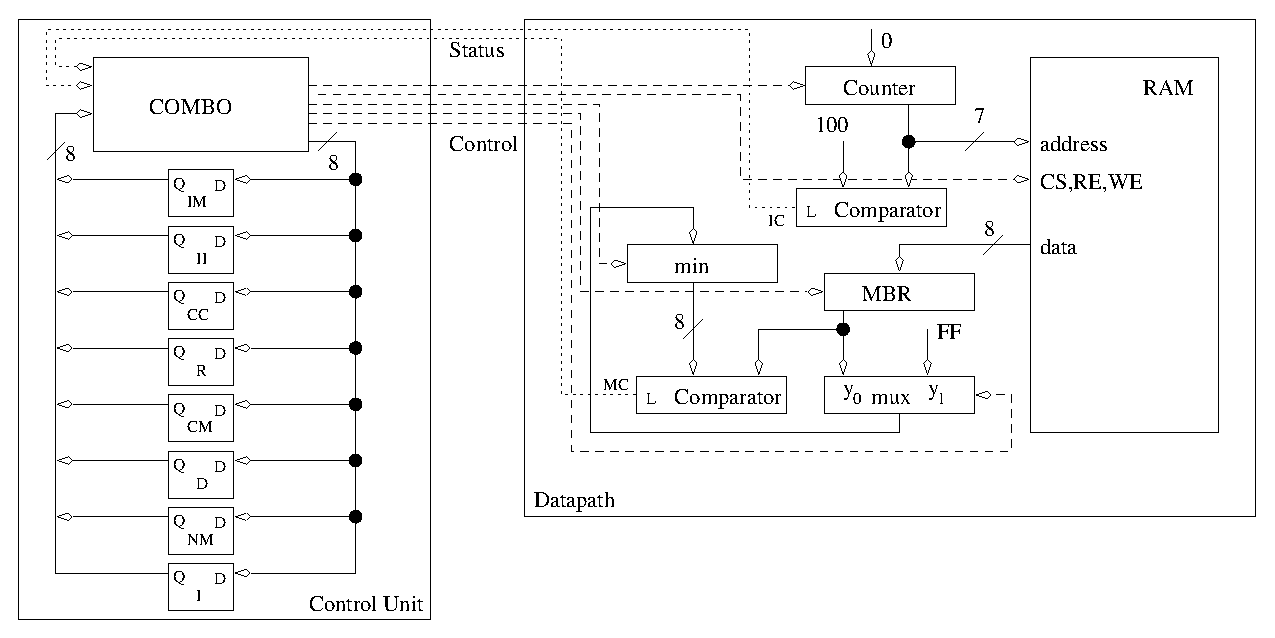
\includegraphics{./Fig8/MinSearch2}} & i
	\scalebox{0.3}{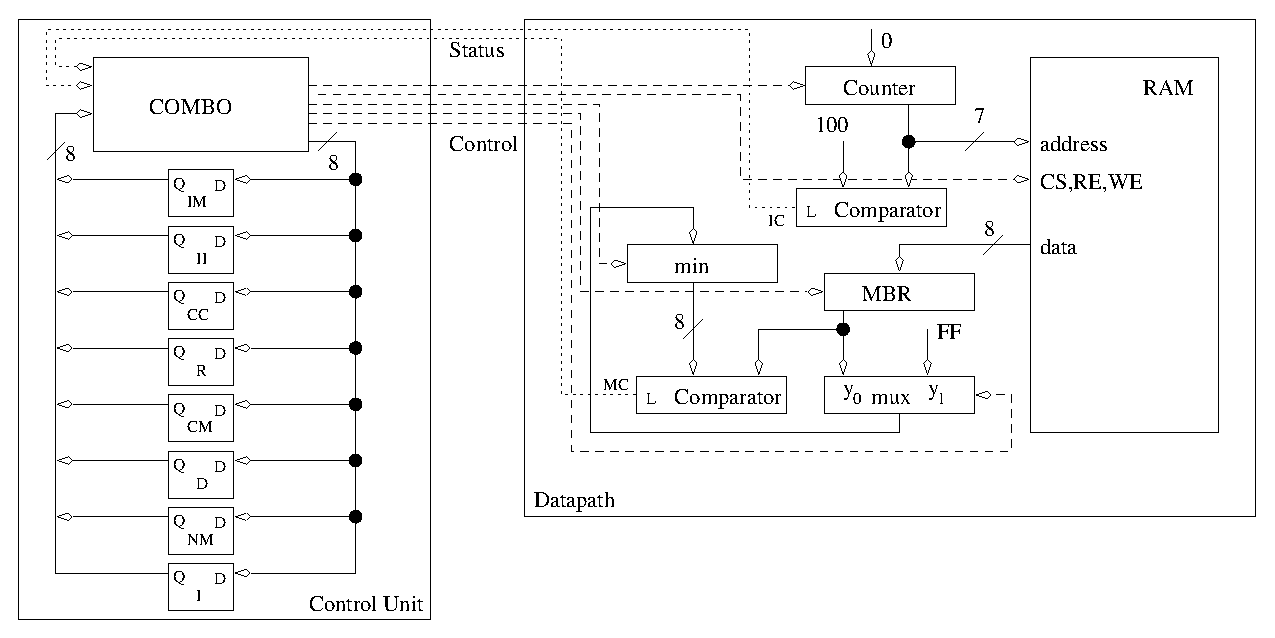
\includegraphics{./Fig8/MinSearch2}} \\
2. State {\bf InitI}   \vspace{10mm}        & 6. State {\bf NewMin} \\
\scalebox{0.3}{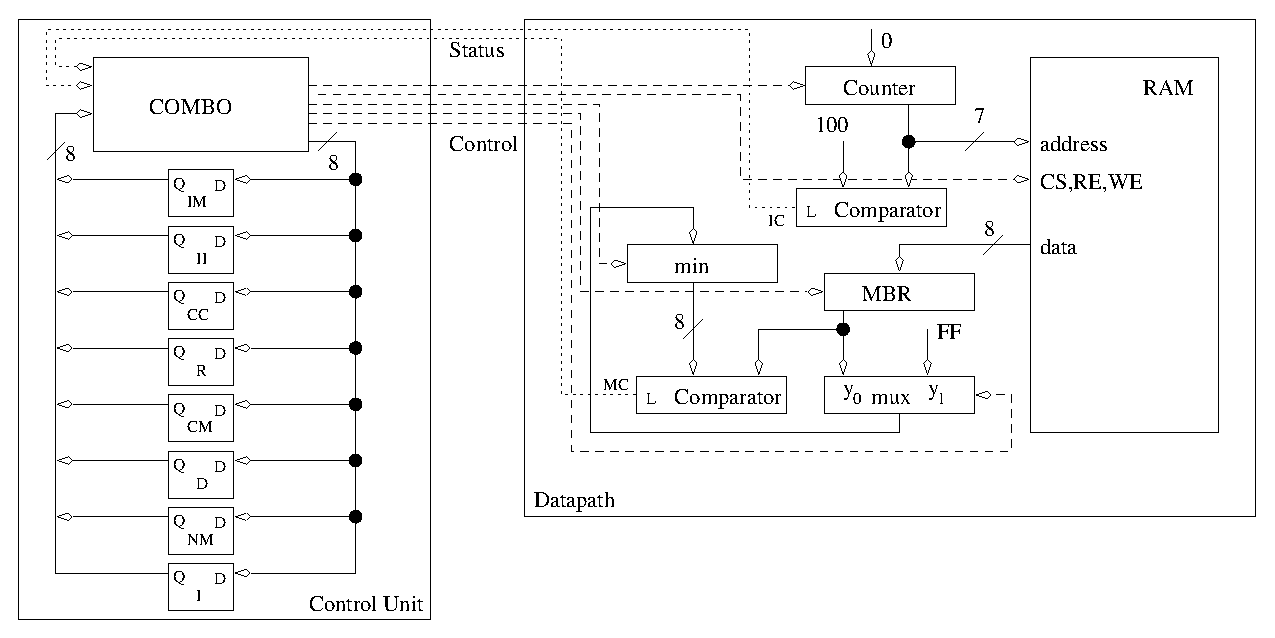
\includegraphics{./Fig8/MinSearch2}} & 
	\scalebox{0.3}{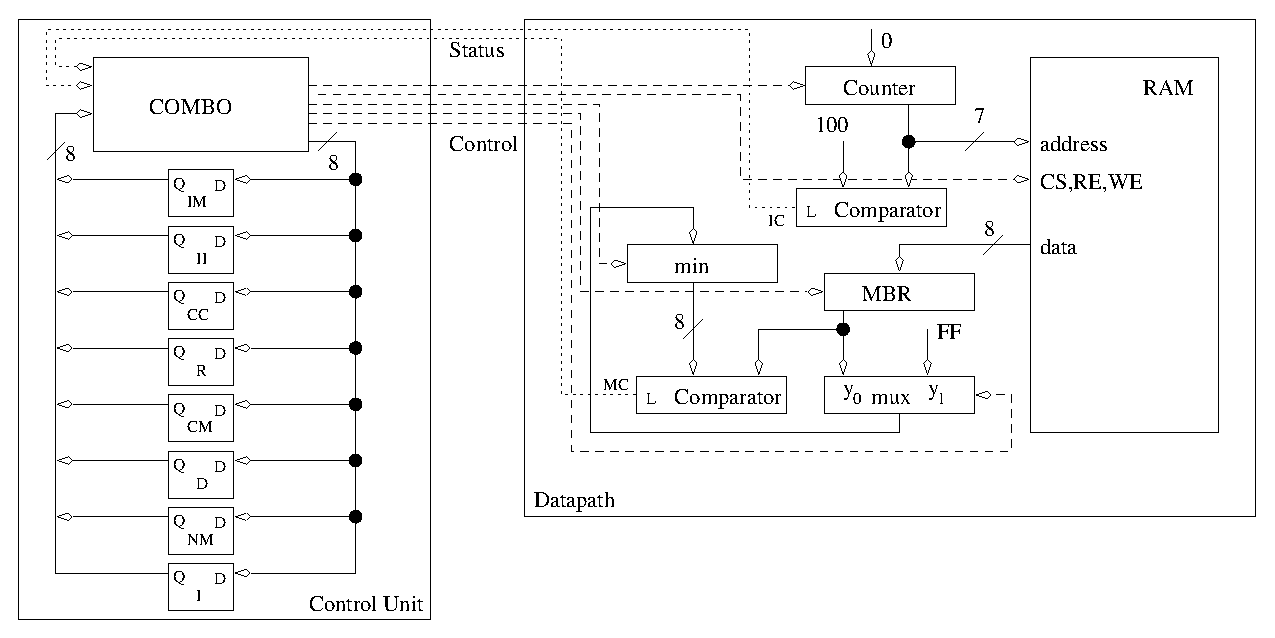
\includegraphics{./Fig8/MinSearch2}} \\
3. State {\bf CompC}   \vspace{10mm}          & 7. State {\bf Inc} \\
\scalebox{0.3}{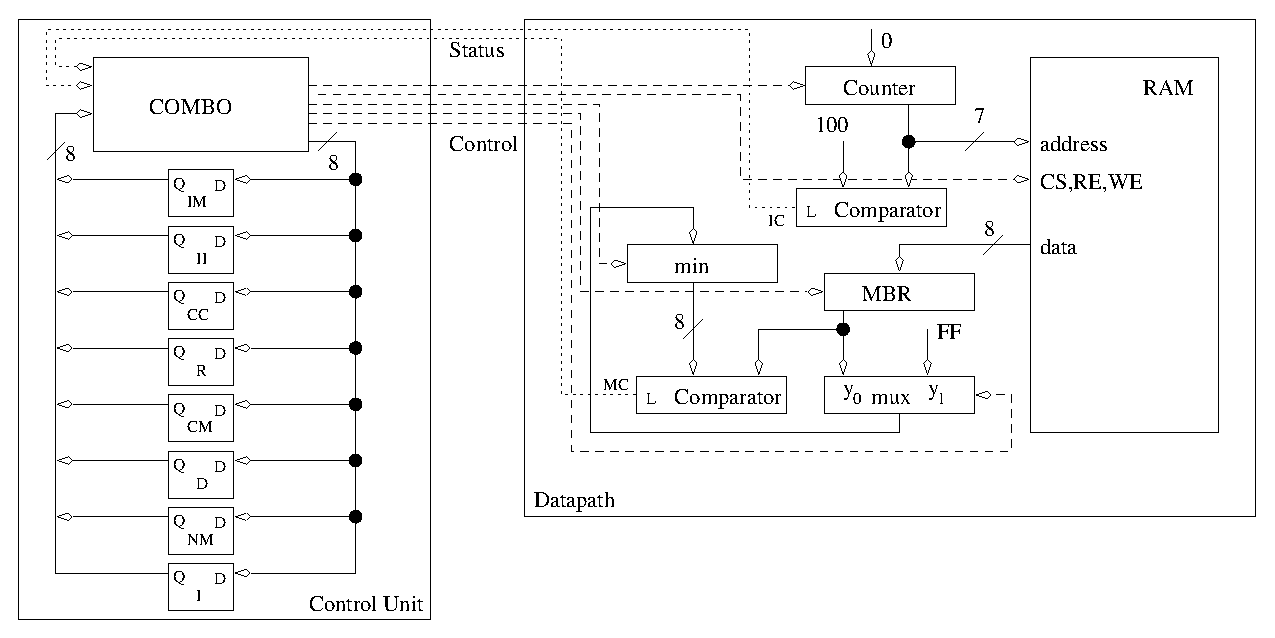
\includegraphics{./Fig8/MinSearch2}} & 
	\scalebox{0.3}{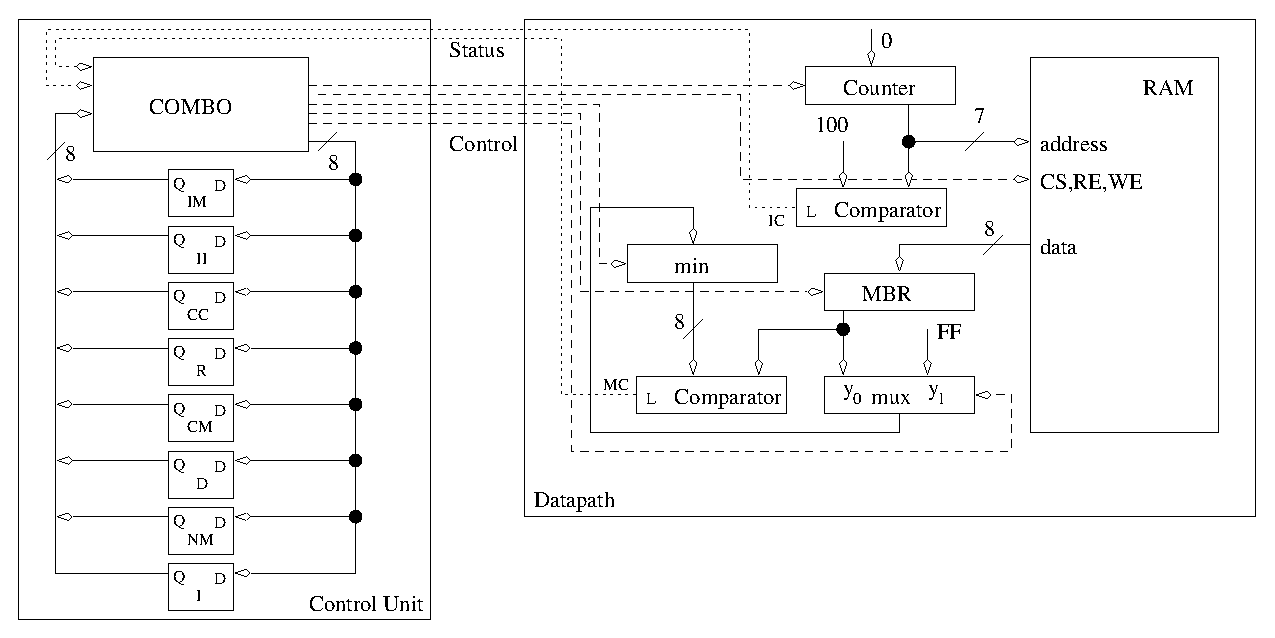
\includegraphics{./Fig8/MinSearch2}} \\
4. State {\bf Read}                                  & 8. State {\bf CompC} \\
\end{tabular}

\pagebreak

\item[Bit Counter]
Design a digital circuit that counts the number of 1's in an
8 bit number X and puts the result into a register Y.
The 8 bit number is provided by an external user using a two-line
handshake protocol. The digital circuit is to play the role of the
passive consumer.  Your circuit should do this task forever.  That
is, after counting the number of 1's, you circuit should read
in a new value of X.


\begin{verbatim}
1.  while(true) {               // Forever
2.      while(REQ==0);          // Wait for the REQ signal
3.      X = data;               // When we get a REQ latch data
4.      ACK = 1;		
5.      while(REQ == 1);        // Wait for REQ to go low
6.      ACK = 0;                // then drop the ACK
7.      Y = 0;                  // Clear the bit count
8.      for (i=0; i<8; i++) {   // For each bit of X
9.          if (X(0) == 1) then // If the LSB of X is a 1  
10              Y = Y + 1;      //   then increment Y
11          X = X >> 1;         // Shift X to the right 1 bit
12      } // end for
13  } // end while
\end{verbatim}

\scalebox{0.7}{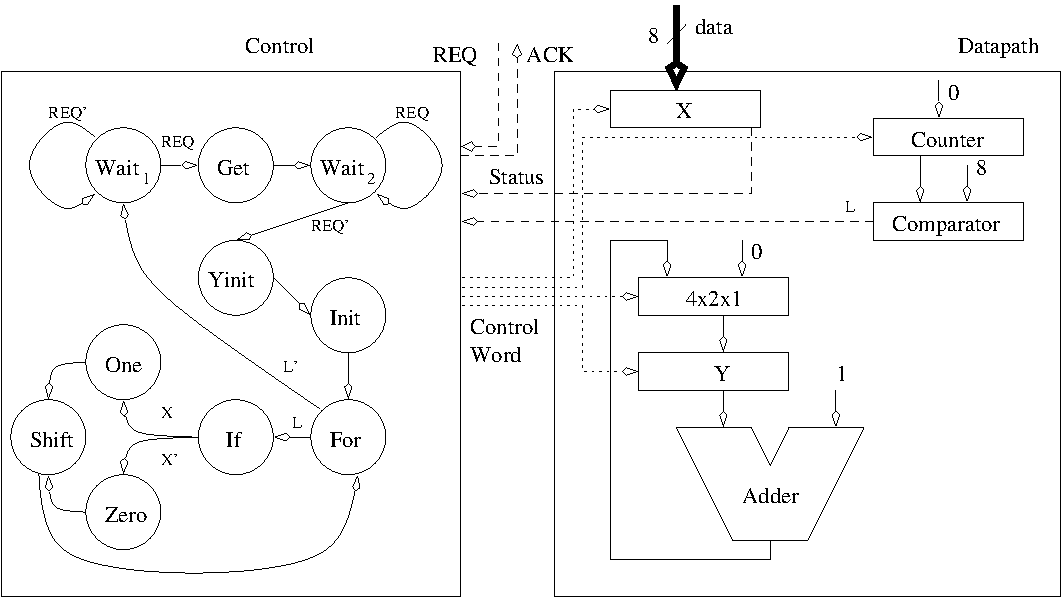
\includegraphics{./Fig8/BitCount1}}

\begin{tabular}{c||c|c|c|c|c}  
State   & ACK       &   X         &  Reg Y    & Y mux         & Counter       \\ \hline
        &           &   00 hold   &  0 hold   & 0 load 0      & 00 hold       \\ \hline
        &           &   01 lsr    &           &               & 01 load       \\ \hline
        &           &   10 lsl    &  1 load   & 1 load Add    & 10 count      \\ \hline
        &           &   11 load   &           &               &               \\ \hline \hline
Wait1   &          &           &          &              &             \\ \hline
Get     &          &           &          &              &             \\ \hline
Wait2   &          &           &          &              &             \\ \hline
Yinit   &          &           &          &              &             \\ \hline
Init    &          &           &          &              &             \\ \hline
For     &          &           &          &              &             \\ \hline
If      &          &           &          &              &             \\ \hline
One     &          &           &          &              &             \\ \hline
Zero    &          &           &          &              &             \\ \hline
Shift   &          &           &          &              &             \\ 
\end{tabular}

\begin{tabular}{p{2in}p{1in}}
$D_{W1} =$	&	$Z_{ACK} =$  		\\
$D_{G} = $	&	$Z_{X} = $		\\
$D_{W2} =$	&	$Z_{RegY} =$  	\\
$D_{YI} =$ 	&	$Z_{Ymux} =$ 		\\
$D_{I} = $	&	$Z_{C1} =$ 		\\
$D_{F} = $	&	$Z_{C0} =$ 		\\
$D_{If} =$ 	&				\\
$D_{One} =$ 	&				\\
$D_{Zer} =$ 	&				\\
$D_{Sft} =$ 	&				\\
\end{tabular}

\pagebreak

\item[RAM counter]
Build a circuit that reads in an 8 bit value, KEY, using a two
line handshake; your circuit is a passive consumer.
Your circuit should search an 8kx8 RAM counting the number
of words that match KEY.  It takes one full clock cycle
to read the RAM.  You may assume that the RAM is pre-loaded
with data.  Your circuit should do this task forever.


\begin{verbatim}
1.    while(1) {
2.        while(REQ == 0);
3.        KEY = data;
4.        ACK = 1;
5.        while(REQ == 1);
6.        ACK = 0;
7.        match = 0;
8.        for(i=0; i<8191; i++) {
9.            MBR = RAM[i]; 
10.            if (MBR == KEY) {
11.                match=match+1;
12.            } // end if
13.        } // end for 
14.    } // end while
\end{verbatim}

\scalebox{0.5}{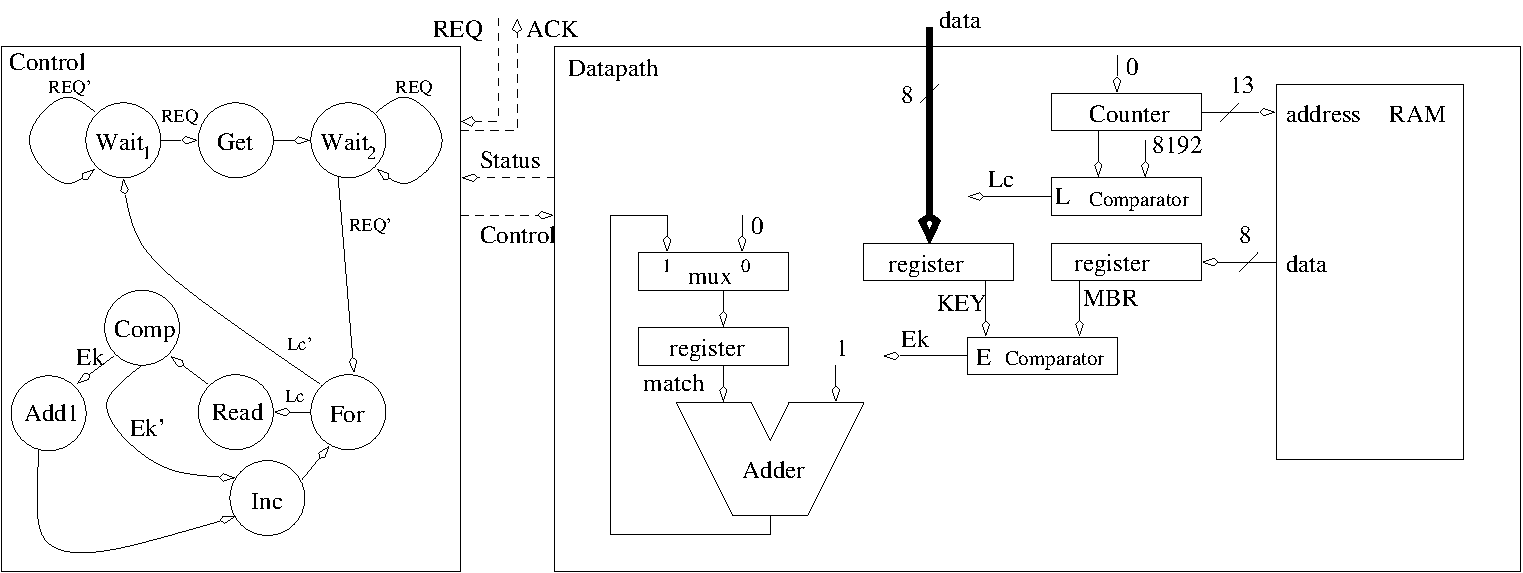
\includegraphics{./Fig8/RAMmatch}}

{\tiny
\begin{tabular}{c||c|c|c|c|c|c|c|c|c}  
State   & ACK   & mux       &  Reg match& Reg KEY & Counter     & MBR    & CS       & RE     & WE       \\ \hline
        & 0     & 0 pass 0  &  0 hold   & 0 hold  & 00 hold     & 0 hold & 0 NULL   & 0 NULL & 0 NULL   \\ \hline
        &       &           &           &         & 01 load     &        &          &        &          \\ \hline
        & 1     & 1 match+1 &  1 load   & 1 load  & 10 count    & 1 load & 1 active & 1 read & 1 write  \\ \hline \hline
Wait1   &      &          &          &        &           &       &         &       &          \\ \hline
Get     &      &          &          &        &           &       &         &       &          \\ \hline
Wait2   &      &          &          &        &           &       &         &       &          \\ \hline
For     &      &          &          &        &           &       &         &       &          \\ \hline
Read    &      &          &          &        &           &       &         &       &          \\ \hline
Comp    &      &          &          &        &           &       &         &       &          \\ \hline
Add1    &      &          &          &        &           &       &         &       &          \\ \hline
Inc     &      &          &          &        &           &       &         &       &          \\ 
\end{tabular} }

\pagebreak

\item [Extra]
Design a circuit that moves $M$ consecutive words from address $S$ (source) to
address $D$ (destination).  For example, if $M=4$, $S=3EA$ and $D=1FE$ then the
circuit would move words 3EA, 3EB, 3EC and 3ED to address 1FE, 1FF, 200 and 201.
Each of $M,S,D$ is preloaded into a register.  While this problem appears simple,
its really rather treacherous.  The circuit will have to handle cases where
$S+M > D$.  In such a case the order of the data movement must be carefully planned.
In order to simplify the design, assume that $S<D$.  Turn in an algorithm,
datapath and control, the
control word, MIEs and OEs.  These circuit will need a three-state buffer to
be able to both read and write to the RAM.  Do not worry about the sizes of the
registers or RAM.


\end{description}
